\section{Procesai ir jų primityvai}
	\subsection{Procesų būsenos}
		\begin{itemize}
			\item \textbf{READY} - procesas, laukiantis procesoriaus.
			\item \textbf{STOPPED} - procesas, sustabdytas kito proceso. 
			\item \textbf{BLOCKED} - procesas, prašantis resurso.
			\item \textbf{RUNNING} - vykdomas procesas.
		\end{itemize}
	\subsection{Būsenų sąryšiai}
		\begin{enumerate}
			\item READY -> RUNNING - paskisrtytojas paskiria procesorių procesui.
			\item READY ->  READY-STOPPED - pasiruošęs procesas buvo sustabdytas einamojo proceso.
			\item READY-STOPPED -> READY - einamasis procesas "nuima" būseną sustabdytas, tačiau jis laukia procesoriaus.
			\item RUNNING -> BLOCKED - procesas užblokuojamas, kai paprašo resurso.
			\item RUNNING -> READY - iš proceso "atimamas" procesorius ir jam netrūksta resursų.
			\item BLOCKED -> BLOCKED-STOPPED - einamasis procesas sustabdo blokuotą procesą.
			\item BLOCKED -> READY - procesas gauna reikiamą resursą.
			\item BLOCKED-STOPPED -> READY-STOPPED - gauna resursą, tačiau procesas vis dar sustabdytas.
			\item BLOCKED-STOPPED -> BLOCKED - einamasis procesas "nuima" būseną sustabdytas, tačiau jam vis dar reikia resurso.
		\end{enumerate}
		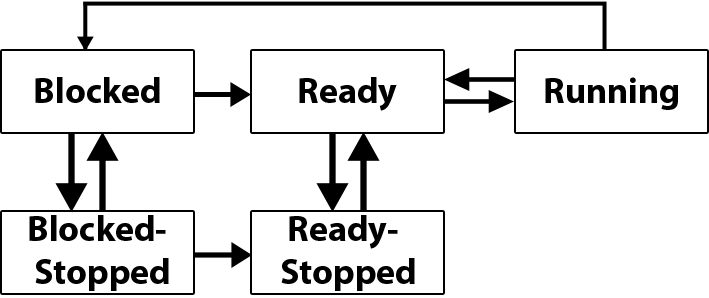
\includegraphics[scale=0.75]{ProcessState.png}
	\subsection{Proceso deskriptorius}
		\begin{itemize}
			\item ID - proceso išorinis vardas.
			\item PID - proceso vidinis vardas.
			\item PPID - proceso tėvo vidinis vardas.
			\item STATE - proceso būsena.
			\item PTR - puslapiavimo lentelės adresas.
			\item RES - laukiamų resursų sąrašas.
			\item REG - registrai (R1,R2,SF,IC) .
			\item CRES - proceso sukurtų resursų sąrašas.
		\end{itemize}
	\subsection{Procesų sąrašai}
		\begin{enumerate}
			\item \textbf{Procesų prioritetų sąrašas} - nurodomas proceso vidinis vardas ir jo prioritetas.
			\item \textbf{Blokuotų procesų sąrašas} - sąrašas užblokuotų procesų.
			\item \textbf{Pasiruošusių procesų sąrašas} - sąrašas pasiruošusių procesų.
			\item  \textbf{Resursų sąrašas} - nurodomas resurso vidinis vardas.
		\end{enumerate}
	\subsection{Prioritetų sudarymo tvarka}
		Prioritetų reikšmės bus skiriamos nuo 0 iki 100. Sisteminiai procesai turės didesnį prioritetą, nei vartotojo. Kiekvieną kartą procesui gavus procesorių, jo prioritetas sumažinamas vienetu. Vartotojas turi galimybę nustatyti prioriteto reikšmę rankiniu būdu (load funkcijos metu).
	\subsection{Sisteminiai procesai}
		Sisteminiai procesai sukuriami paleidžiant sistemą, o sunaikinami tik sistemai baigus darbą. Jie yra pasiruošę dirbti visą sistemos gyvavimo laiką. 
	
		\begin{tabular}{|p{1cm} | *{2}{p{3.4cm} |} p{7.5cm} |}
				\hline
				ID	& Pavadinimas		& Prioritetas	& Aprašymas\\
				\hline
				1	& Start\_Stop		& 100			& Visų procesų tėvinis procesas; kuria ir naikina sisteminius procesus ir resursus. Visalaiką užsiblokavęs, kol dirba OS\\
				\hline
				2	& Job\_Governor		& 99			& Procesų paskirstytojas, tvarkantis virtualių mašinų darbą.\\
				\hline
				3	& Loader			& 96			& Užkrauna procesą iš išorinės atminties į vidinę atmintį.\\
				\hline
				4	& Chan\_1\_Device	& 90			& Perrašo duomenis tarp išorinės atminties ir vidinės atminties.\\
				\hline
				5	& Interrupt			& 98			& Procesas, kuris, įvykus pertraukimui, jį identifikuoja ir siunčia pranešimą Job\_Governor.\\
				\hline
				6	& Get\_Put\_Data	& 85			& Procesas, dirbantis su duomenimis vidinėje atmintyje.\\
				\hline
				7	& Chan\_2\_Device	& 70			& Darbui su įvesties srautais.\\
				\hline
				8	& Chan\_3\_Device	& 65			& Darbui su išvesties srautais.\\
				\hline
				9	& Process\_Killer	& 89			& Ištrina programą ir jos sukurtus resursus iš vidinės atminties.\\
				\hline
				10	& Resource\_Manager	& 93			& Resursų paskirstytojas.\\
				\hline
				11	& JCL				& 69 			& \textbf{J}ob \textbf{C}ontrol \textbf{L}anguage procesas gauna blokus iš Chan\_2\_Device ir peržiūri, ar programos kodo struktūra yra korektiška; jei taip, perduoda programos blokų sąrašą Chan\_1\_Device.\\
				\hline
				12	& VM				& 50			& Procesas, skirtas vykdyti vartotojo programą tol, kol aptinkamas pertraukimas.\\
				\hline
		\end{tabular}
	\subsection{Procesų planuotojas (Job\_Governor)}
		Procesų planuotojas iškviečiamas kiekvieną kartą, kai iššaukiamas timer'io pertraukimas. Taip pat jis gali būti kviečiamas procesui baigus darbą arba jam užsiblokavus. Iškvietus planuotoją, imamas kitas READY būsenos procesas pagal didžiausią prioritetą.
	\subsection{Procesų planuotojo primityvai}
		\begin{enumerate}
			\item \textbf{Kurti procesą} - šiam primityvui perduodama nuoroda į jo tėvą, pradinė proceso būsena, jo prioritetas, vidinis vardas. Primityvo viduje kuriamas procesas, jis įdedamas į atitinkamus sąrašus (pasiruošusių/blokuotų), sukuriamas jo vaikų sąrašas.
			\item \textbf{Naikinti procesą} - pirmiausia sunaikinami proceso sukurti vaikiniai procesai bei resursai. Tada procesas pašalinamas iš sąrašų, kuriems jis priklauso. Pabaigoje sunaikinami procesui perduoti resursai ir jo pačio deskriptorius.
			\item \textbf{Stabdyti procesą} - proceso būsena pakeičiama iš BLOCKED į BLOCKED-STOPPED arba iš READY į READY-STOPPED.
			\item  \textbf{Aktyvuoti procesą} - būsena keičiama iš BLOCKED-STOPPED į BLOCKED arba iš READY-STOPPED į READY.
		\end{enumerate}
	\clearpage